\documentclass[a5paper, 10pt]{article}

% Текст
\usepackage[utf8]{inputenc} % UTF-8 кодировка
\usepackage[russian]{babel} % Русский язык
\usepackage{indentfirst} % красная строка в первом параграфе в главе
% Отображение страниц
\usepackage{geometry} % размеры листа и отступов
\usepackage{listings}
\usepackage{color}

\geometry{
	left=12mm,
	top=25mm,
	right=15mm,
	bottom=17mm,
	marginparsep=0mm,
	marginparwidth=0mm,
	headheight=10mm,
	headsep=7mm,
	nofoot}
\usepackage{afterpage,fancyhdr} % настройка колонтитулов
\pagestyle{fancy}
\fancypagestyle{style}{ % создание нового стиля style
	\fancyhf{} % очистка колонтитулов
	\fancyhead[LO, RE]{Лабораторная работа № 5 } % название документа наверху
	\fancyhead[RO, LE]{Задачи 1067, 1521, 1628} % название section наверху
	\fancyfoot[RO, LE]{\thepage} % номер страницы справа внизу на нечетных и слева внизу на четных
	\renewcommand{\headrulewidth}{0.25pt} % толщина линии сверху
	\renewcommand{\footrulewidth}{0pt} % толцина линии снизу
}
\fancypagestyle{plain}{ % создание нового стиля plain -- полностью пустого
	\fancyhf{}
	\renewcommand{\headrulewidth}{0pt}
}
\fancypagestyle{title}{ % создание нового стиля title -- для титульной страницы
	\fancyhf{}
	\fancyhead[C]{{\footnotesize
			Министерство образования и науки Российской Федерации\\
			Федеральное государственное автономное образовательное учреждение высшего образования
	}}
	\fancyfoot[C]{{\large 
			Санкт-Петербург, 2024
	}}
	\renewcommand{\headrulewidth}{0pt}
}

% Математика
\usepackage{amsmath, amsfonts, amssymb, amsthm} % Набор пакетов для математических текстов
%\usepackage{dmvnbase} % мехматовский пакет latex-сокращений
\usepackage{cancel} % зачеркивание для сокращений
% Рисунки и фигуры
\usepackage[pdftex]{graphicx} % вставка рисунков
\usepackage{wrapfig, subcaption} % вставка фигур, обтекая текст
\usepackage{caption} % для настройки подписей
\captionsetup{figurewithin=none,labelsep=period, font={small,it}} % настройка подписей к рисункам
% Рисование
\usepackage{tikz} % рисование
\usepackage{circuitikz}
\usepackage{pgfplots} % графики
% Таблицы
\usepackage{multirow} % объединение строк
\usepackage{multicol} % объединение столбцов
% Остальное
\usepackage[unicode, pdftex]{hyperref} % гиперссылки
\usepackage{enumitem} % нормальное оформление списков
\setlist{itemsep=0.15cm,topsep=0.15cm,parsep=1pt} % настройки списков
% Теоремы, леммы, определения...
\theoremstyle{definition}
\newtheorem{Def}{Определение}
\newtheorem*{Axiom}{Аксиома}
\theoremstyle{plain}
\newtheorem{Th}{Теорема}
\newtheorem{Lem}{Лемма}
\newtheorem{Cor}{Следствие}
\newtheorem{Ex}{Пример}
\theoremstyle{remark}
\newtheorem*{Note}{Замечание}
\newtheorem*{Solution}{Решение}
\newtheorem*{Proof}{Доказательство}
% Свои команды
\newcommand{\comb}[1]{\left[\hspace{-4pt}\begin{array}{l}#1\end{array}\right.\hspace{-5pt} } % совокупность уравнений
% Титульный лист
\usepackage{csvsimple-l3}
\newcommand*{\titlePage}{
	\thispagestyle{title}
	\begingroup
	\begin{center}
		%		{\footnotesize
			%			Министерство образования и науки Российской Федерации\\
			%			Федеральное государственное автономное образовательное учреждение высшего образования
			%		}
		%		
		\vspace*{6ex}
		
		{\small
			САНКТ-ПЕТЕРБУРГСКИЙ НАЦИОНАЛЬНЫЙ ИССЛЕДОВАТЕЛЬСКИЙ УНИВЕРСИТЕТ ИТМО	
		}
		
		\vspace*{2ex}
		
		{\normalsize
			Факультет систем управления и робототехники
		}
		
		\vspace*{15ex}
		
		{\Large \bfseries 
			Лабораторная работа № 5
		}
\vspace*{2ex}
	{\Large \bfseries 
			
"Задачи 1067, 1521, 1628"
		}
\vspace*{2ex}
		
		{\normalsize
			по дисциплине Алгоритмы и структуры данных
		}

	\end{center}
	\vspace*{20ex}
	\begin{flushright}
		{\large 
			\underline{Выполнила}: студентка гр. \textbf{R3238}\\
                             поток \textbf{2.1}\\
			\begin{flushright}
				\textbf{Нечаева А. А.}\\
			\end{flushright}
		}
		
		\vspace*{5ex}
		
		{\large 
			\underline{Преподаватель}: \textit{Тропченко Андрей Александрович}
		}
	\end{flushright}	
	\newpage
	\setcounter{page}{1}
	\endgroup}

\begin{document}
	\titlePage
	\pagestyle{style}

\lstset{ %
language=C,                 % выбор языка для подсветки (здесь это С)
basicstyle=\small\sffamily, % размер и начертание шрифта для подсветки кода
numbers=left,               % где поставить нумерацию строк (слева\справа)
numberstyle=\tiny,           % размер шрифта для номеров строк
stepnumber=1,                   % размер шага между двумя номерами строк
numbersep=5pt,                % как далеко отстоят номера строк от подсвечиваемого кода
backgroundcolor=\color{white}, % цвет фона подсветки - используем \usepackage{color}
showspaces=false,            % показывать или нет пробелы специальными отступами
showstringspaces=false,      % показывать или нет пробелы в строках
showtabs=false,             % показывать или нет табуляцию в строках
frame=single,              % рисовать рамку вокруг кода
tabsize=2,                 % размер табуляции по умолчанию равен 2 пробелам
captionpos=t,              % позиция заголовка вверху [t] или внизу [b] 
breaklines=true,           % автоматически переносить строки (да\нет)
breakatwhitespace=false, % переносить строки только если есть пробел
escapeinside={\%*}{*)}   % если нужно добавить комментарии в коде
}



\newpage
\section{Цель}
Разработать и реализовать алгоритмы для решения задач 1067, 1521 и 1628.


\section{Задача 1067}

\begin{figure}[h!]
\center{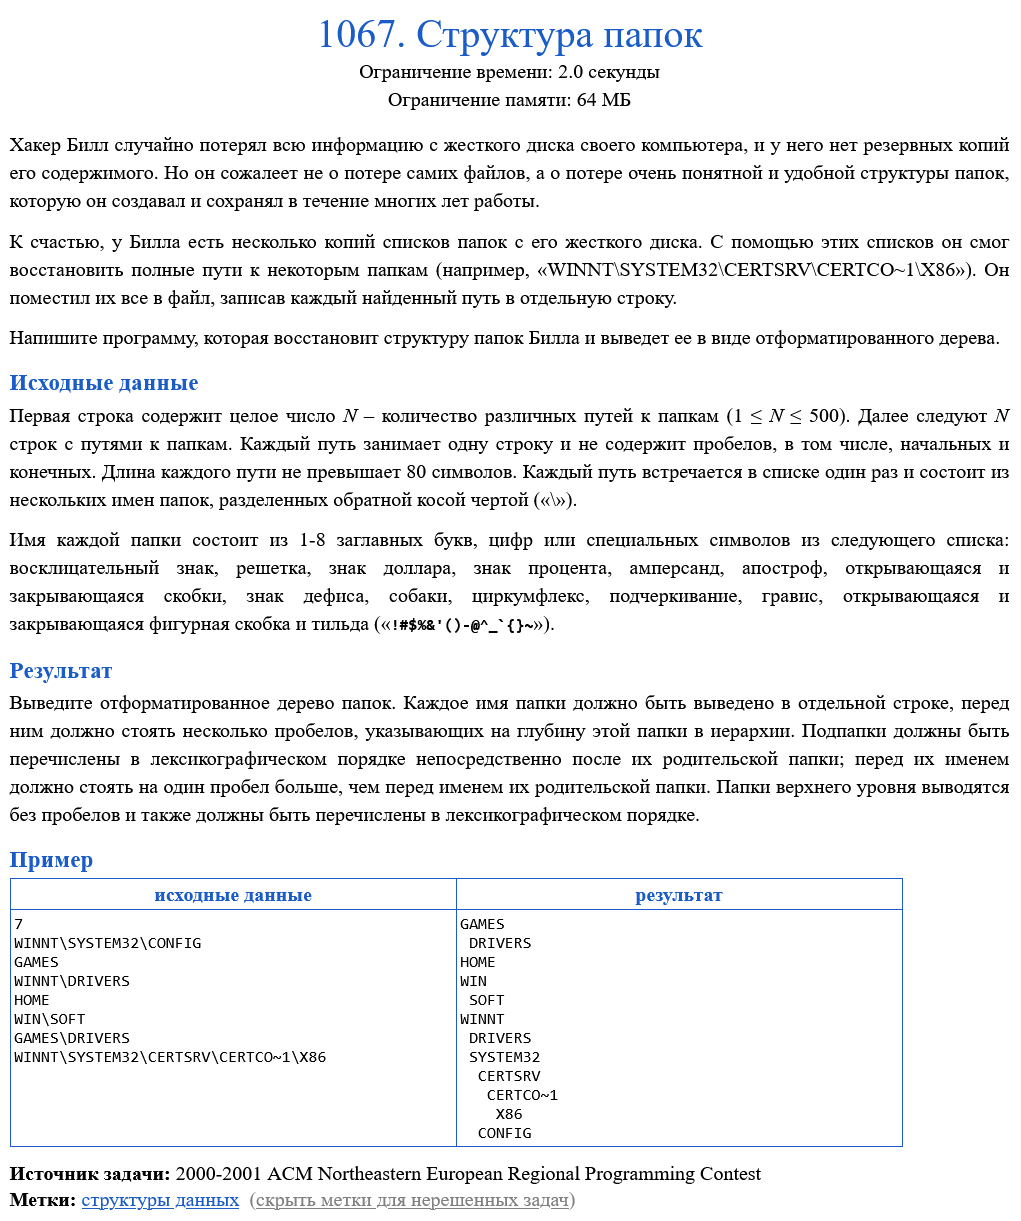
\includegraphics[width=0.8\linewidth]{pic/task_1067.png}}
\caption{Условие задачи 1067.}
\end{figure}

\subsection{Краткое описание алгоритма}
\textbf{1. Входные данные:} первая строка содержит целое число $N$ $-$ количество путей к папкам $(1 \leq N \leq 500)$. Дальше следуют $N$ строк с путями к папкам. Каждый путь занимает одну строку и не содержит пробелов, в том числе, начальных и конечных. Длина каждого пути не превышает $80$ символов. Каждый путь встречается в списке один раз и состоит из нескольких имен папок, разделенных обратной косой чертой ("$\backslash$"). \\
Имя каждой папки состоит из 1-8 заглавных букв, цифр или специальных символов из следующего списка: восклицательный знак, решетка, знак доллара, знак процента, амперсанд, апостроф, открывающаяся и закрывающаяся скобки, знак дефиса, собаки, циркумфлекс, подчеркивание, гравис, открывающаяся и закрывающаяся фигурная скобка и тильда. \\
\textbf{2.} Прямая реализация описанного в задании алгоритма действий с помощью специальной структуры, содержащей имя и указатели на дочерние каталоги; \\
\textbf{3.} После реализован рекурсивный обход полученной структуры директорий в глубину. \\
\textbf{4.}  И с помощью отдельного метода выведен результат.\\
\textbf{5.} Выходные данные: вывести отформатированное дерево папок. Каждое имя папки должно быть выведено в отдельной строке, перед ним должно стоять несколько пробелов, указывающих на глубину этой папки в иерархии. Подпапки должны быть перечислены в лексикографическом порядке непосредственно после их родительской папки; перед их именем должно стоять на один пробел больше, чем перед именем их родительской папки. Папки верхнего уровня выводятся без пробелов и также должны быть перечислены в лексикографическом порядке.

\subsection{Листинг}

\begin{center}
\begin{lstlisting}[label=some-code,caption={Исходный код для 1067}]
#include <iostream>
#include <map>
#include <utility>


// structure for smart store disk items and their relates
struct disk {
    std::string item;
    std::map<std::string, disk *> child;

    // clang-tidy recommendation for single-argument constructions
    explicit disk(std::string name) {
        // clang-tidy recommendation
        this -> item = std::move(name);
        this -> child = {};
    }

    disk() {
        this -> item = "";
        this -> child = {};
    }
};


// method for printing disk structure in recursive mode
void disk_printer(disk* cur, int depth) {
    for (int i = 0; i < depth - 1; ++i) {
        std::cout << " ";
    }
    if (!cur -> item.empty()) {
        std::cout << cur -> item << std::endl;
    }
    ++depth;

    for (auto &child_dir : cur -> child) {
        disk_printer(child_dir.second, depth);
    }
}


int main() {
    int n;
    std::cin >> n;

    disk* rt = new disk();

    for (int i = 0; i < n; ++i) {
        std::string cur_path;
        std::cin >> cur_path;
        disk* cur_d = rt;
        std::string d;

        for (int j = 0; j <= cur_path.size(); ++j) {
            
            if (cur_path[j] == '\\' || cur_path[j] == '\0') {
                auto d_disk = cur_d -> child.find(d);

                if (d_disk == cur_d -> child.end()) {
                    disk* new_disk = new disk(d);
                    cur_d -> child[d] = new_disk;
                    cur_d = cur_d -> child.find(d) -> second;
                    
                } else {
                    cur_d = d_disk -> second;
                }
                
                d = "";
                
            } else {
                d += cur_path[j];
            }
        }
    }
    disk_printer(rt, 0);

    return 0;
}




\end{lstlisting}
\end{center}

\subsection{Результат}
\begin{figure}[h!]
\center{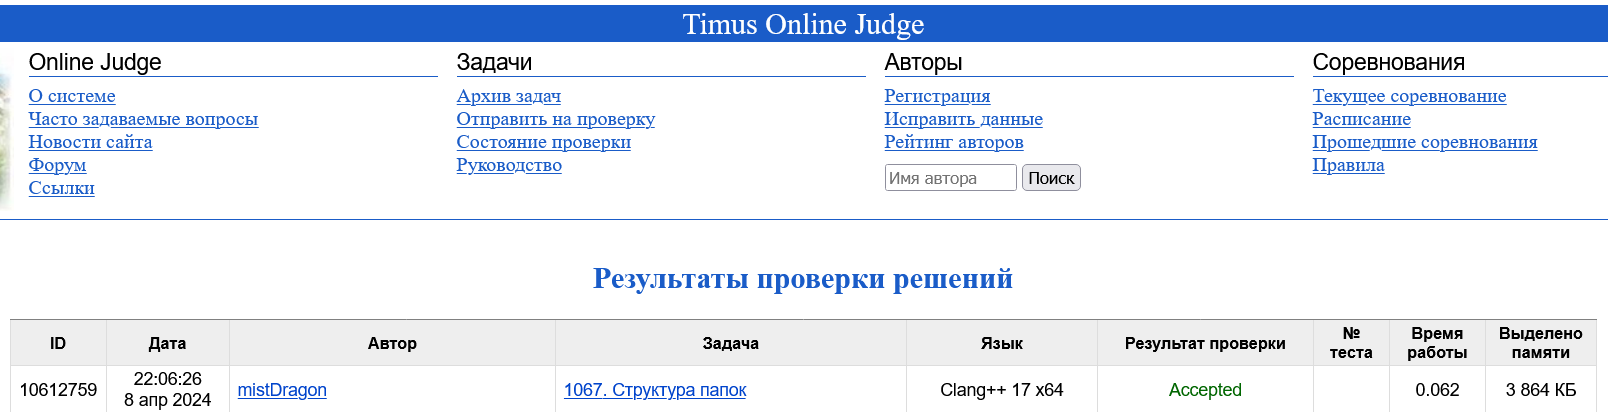
\includegraphics[width=0.9\linewidth]{pic/screen_1067.png}}
\caption{Результат отправки задачи 1067.}
\end{figure}




\newpage
\section{Задача 1521}

\begin{figure}[h!]
\center{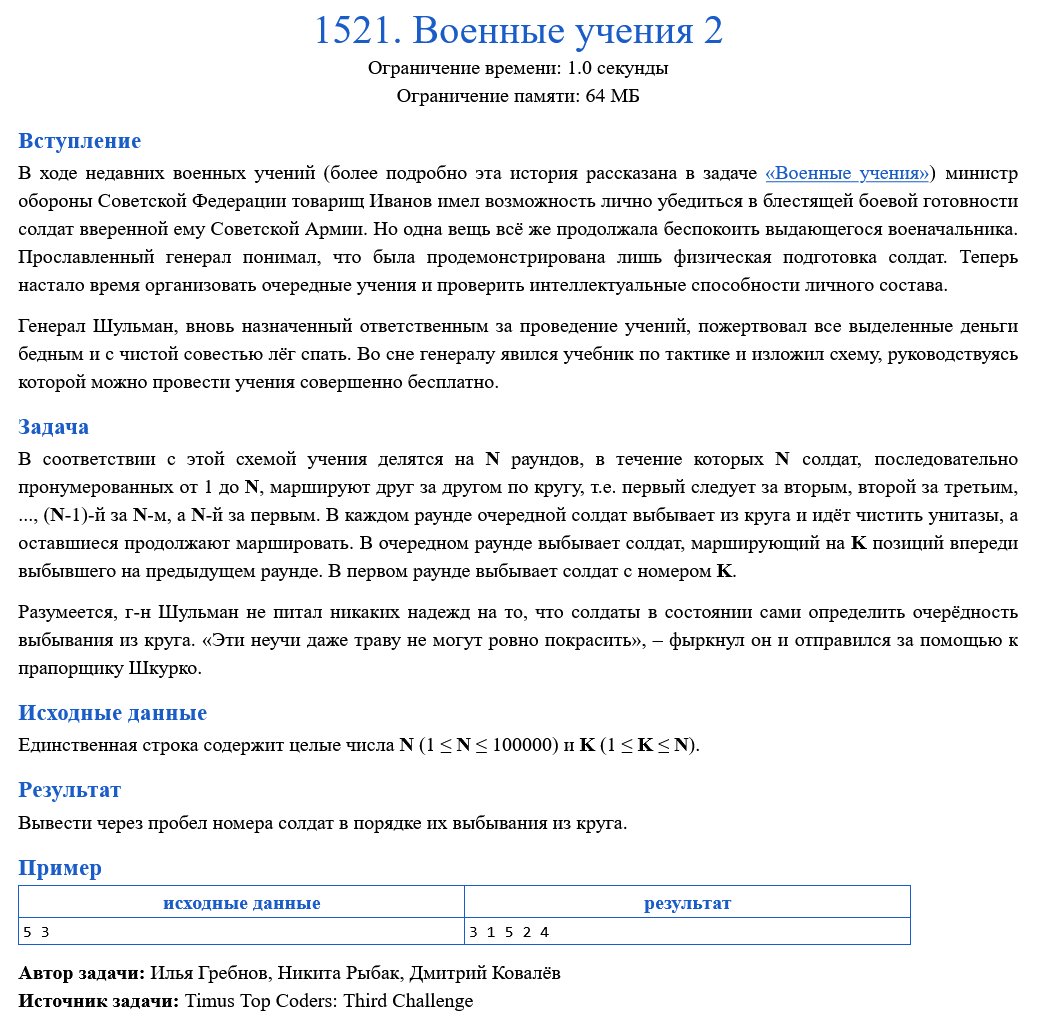
\includegraphics[width=1\linewidth]{pic/task_1521.png}}
\caption{Условие задачи 1521.}
\end{figure}

\subsection{Краткое описание алгоритма}
\textbf{1. Входные данные:} единственная строка содержит целые числа $N\, (1 \leq N \leq 100000)$ и $K \, (1 \leq K \leq N)$. \\
\textbf{2.}  \\
\textbf{3.}  \\
\textbf{4.}  \\
\textbf{5.} Выходные данные: вывести через пробел номера солдат в порядке их выбывания из круга




\subsection{Листинг}

\begin{center}
\begin{lstlisting}[label=some-code,caption={Исходный код для 1521}]
#include <iostream>


\end{lstlisting}
\end{center}

\subsection{Результат}
%\begin{figure}[h]
%\center{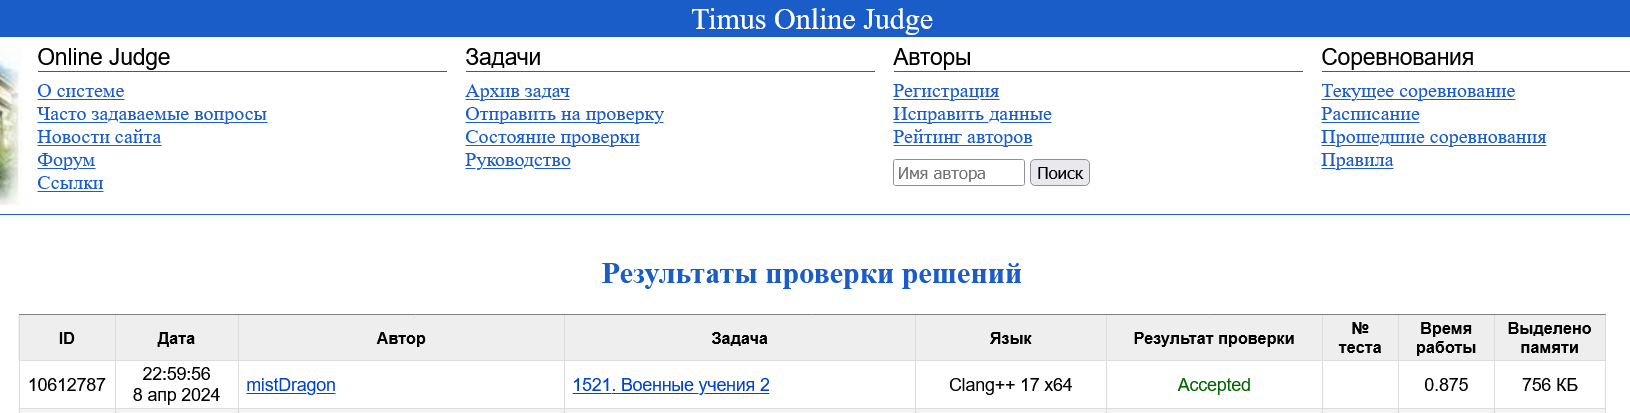
\includegraphics[width=0.9\linewidth]{pic/screen_1521.png}}
%\caption{Результат отправки задачи 1521.}
%\end{figure}




\newpage
\section{Задача 1628}

\begin{figure}[h!]
\center{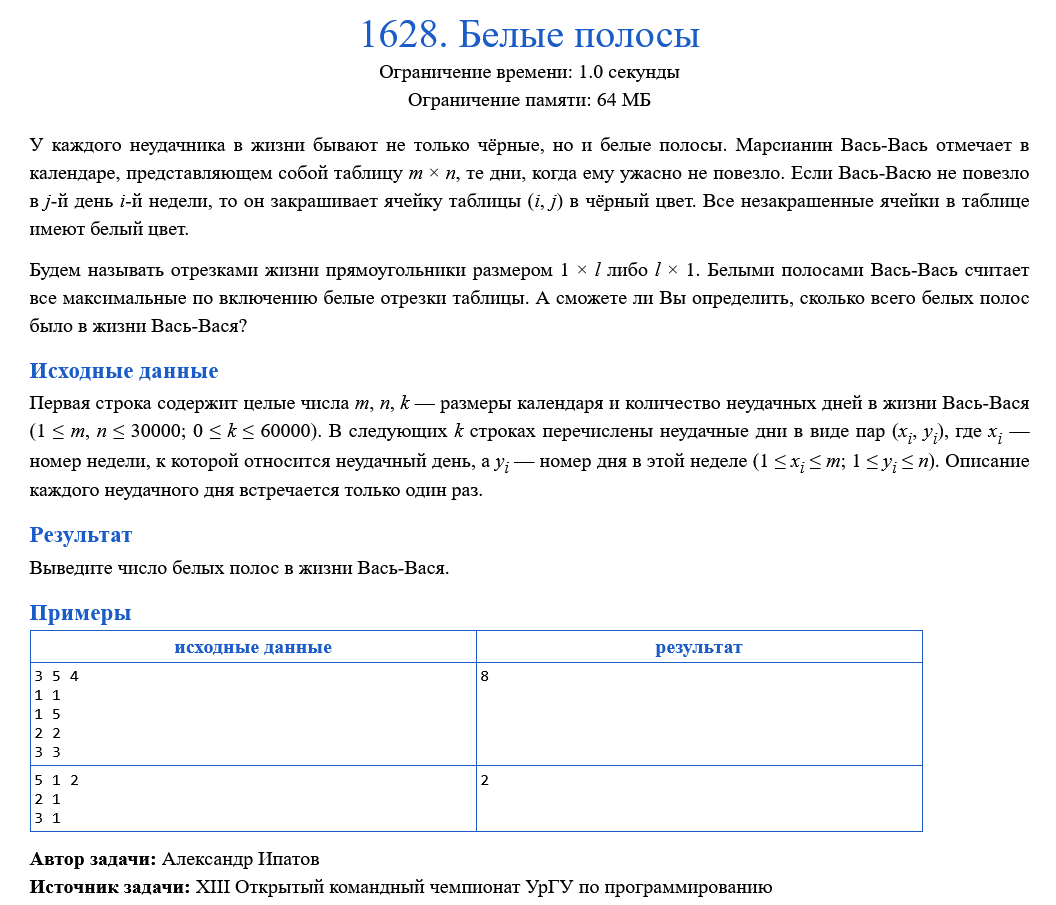
\includegraphics[width=1\linewidth]{pic/task_1628.png}}
\caption{Условие задачи 1628.}
\end{figure}

\subsection{Краткое описание алгоритма}
\textbf{1. Входные данные:} первая строка содержит целые числа $m, \, n, \, k$ $-$ размеры календаря и количество неудачных дней в жизни Вась-Вася $(1 \leq m, n \leq 30000; \, 0 \leq k \leq 60000)$. В следующих $k$ строках календаря перечислены неудачные дни в виде пар $(x_i, y_i)$, где $x_i$ $-$ номер недели, к которой относится неудачный день, а $y_i$ $-$ номер дня в этой неделе $(1 \leq x_i \leq m; \, 1 \leq y_i \leq n)$. Описание каждого неудачного дня встречается только один раз. \\
\textbf{2.}  \\
\textbf{3.}  \\
\textbf{4.}  \\
\textbf{5.} Выходные данные: вывести число белых полос в жизни Вась-Вася.
\subsection{Листинг}

\begin{center}
\begin{lstlisting}[label=some-code,caption={Исходный код для 1628}]
#include <iostream>


\end{lstlisting}
\end{center}

\subsection{Результат}
%\begin{figure}[h]
%\center{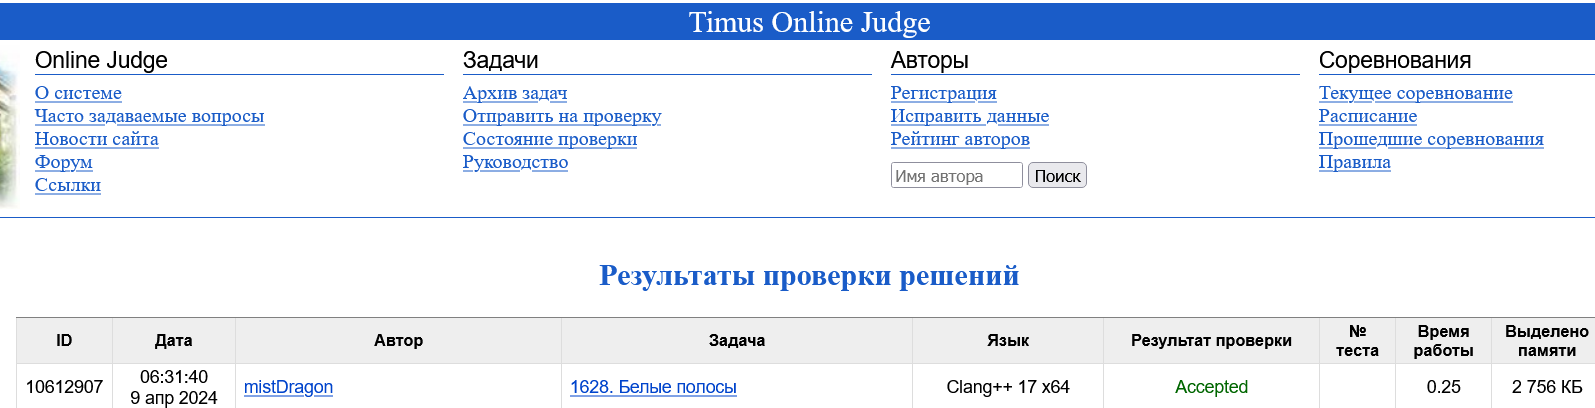
\includegraphics[width=0.9\linewidth]{pic/screen_1628.png}}
%\caption{Результат отправки задачи 1628.}
%\end{figure}



\newpage
\section{Вывод по работе}
В ходе выполнения данной лабораторной работы были реализованы алгоритмы для решения задач $1067$, $1521$ и $1628$. 
\end{document}













